\section{进程与调度分析}

\subsection{进程的概念}

程序与进程的概念是不可分的。当用户在计算机上运行一个程序时,此程序对应的进程就诞生了,并实际完成各种程序提供的功能,而用户关闭一个程序时,进程也随之终止。程序是为了完成某项任务编排的语句序列,它要告诉计算机如何执行,因此程序是需要通过CPU来运行的,且在程序的运行过程中需要占有计算机的各种资源(比如内存等)才能运行下去。

如果计算机系统在任一时刻限制只有一个程序在运行,则程序在整个运行过程中独占计算机中的全部资源,这样整个程序运行和管理就简单了。就象在一个家中只住了一个人A,他想看书就到书房去看书,想睡觉就到睡房的床上去睡觉,想看电视就到电视厅看电视,想吃饭就去餐厅吃饭,没人和他抢占资源。但为了提高计算机系统的资源利用率,需要支持多个程序并发执行。这就会带来许多新的问题,如资源的共享与竞争,同步与互斥等。

比如此人与B成家并有了小孩C,那就是三口之家同时住一套房,当A想去看足球比赛直播电视节目的时候,如果发现电视厅已经有B在坐着看连续剧电视节目了,A就得等待或干别的事情。除非A在买一个电视,并在另外一个房间看他的球比赛直播。

由于程序是静态的,我们看到的程序是存储在存储介质(如硬盘、光盘等)上的,它无法反映出程序执行过程中的动态特性,而且程序在执行过程中会不断申请资源或释放资源,这样让程序作为共享资源的基本单位是不合适的,所以需要引入一个概念,它能描述程序的执行过程而且可以作为共享资源的基本单位,这个概念就是进程。简单地说,一个进程是一个具有一定独立功能的程序在一个数据集合上的一次动态执行过程。每个进程都是整个应用的某一部分。操作系统在逻辑上维护了进程的运行状态信息,即与进程运行直接相关的CPU寄存器和栈空间(只有这样才能实现进程切换)。操作系统根据当前进程的情况设置进程的状态,并根据进程的状态(比如优先级)进行选择一个进程占用CPU并运行,这个过程成为调度。

\subsection{进程控制块}

程序的运行是通过进程体现的,操作系统对进程进行管理和控制,那么操作系统怎么了解到进程的状态并掌握进程占有的资源分配呢,而且进程做状态转换时CPU的现场保存在那呢?这实际是通过进程控制快(Process Control Block, 简称PCB)。PCB是进程 的唯一标志,在其中记录了进程的全部信息,相当于进程的档案。操作系统通过PCB感知进程的存在,通过PCB了解进程和控制 进程的运行。在xv6中,所有的CPU共享一个进程控制块池,即源代码中为proc.c中的proc(即进程控制块)数组。在这 个进程数组保存的进程控制块结构分成两类:一类是未使用的进程控制块结构,另一类是正在使用的进程控制块结构。每次要创建一个进程时,只需要从进程控制块数组中取得一个未使用进程控制块结构进行相应的处理即可。

xv6中结构体 struct proc包含进程大小、页表、内核栈、进程状态、进程id、父进程、目录等等,代码如下:

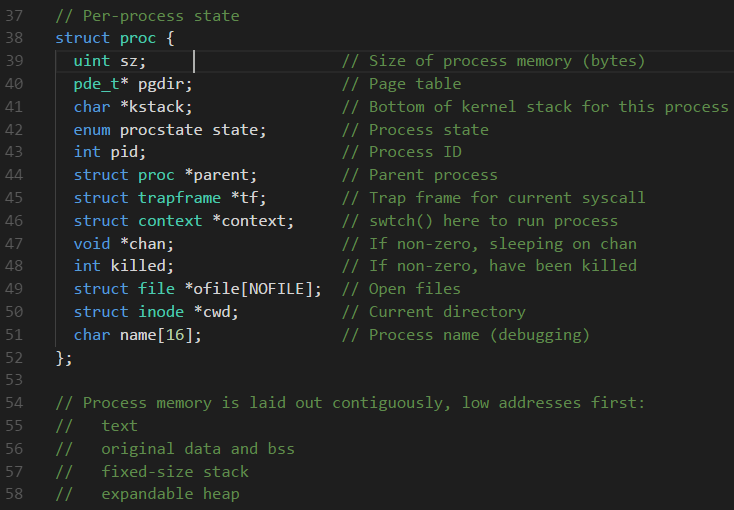
\includegraphics[width=6in]{figures/process/fig2.png}

\begin{itemize}
\item sz是记录进程所占有的内存空间大小;
\item pgdir记录了进程页表的线性地址
\item kstack是进程在内核态的栈;
\item 枚举类型变量 state记录了进程的状态;
\item pid是进程的ID;
\item parent记录父进程;
\item tf是当前系统调用的中断帧;
\item context是切换进程需要维护的硬件寄存器内容, 是进程运行的入口;
\item chan不为NULL时,是进程睡眠时所挂的睡眠队列;
\item killed不为0时,表示进程被杀死了;
\item ofile数组是进程打开的文件数组;
\item cwd是进程运行时所处的当前目录;
\item name保存了进程的名字(用于调试)。
\end{itemize}

struct proc在proc.h中,并且在该文件之中定义了几个关键的数据结构。其中context是在内核进行上下文切换需要保存的寄存器: edi,esi,ebx,ebp,eip.

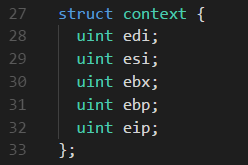
\includegraphics[width=6in]{figures/process/fig3.png}

proc[NPROC]数组(在proc.c文件的12行)定义了xv6所能够支持的进程所需的相关数据,NPROC表示了xv6可支持进程个数。

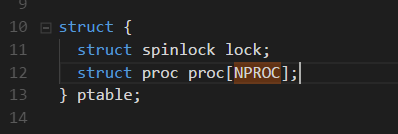
\includegraphics[width=6in]{figures/process/fig4.png}

cpu结构是记录计算机中所有CPU的相关信息:

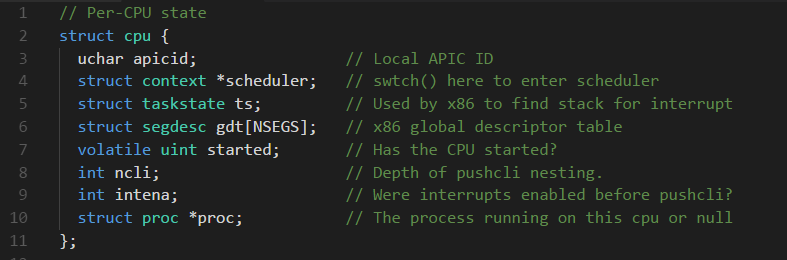
\includegraphics[width=6in]{figures/process/fig5.png}

其中:

\begin{itemize}
\item apicid 代表此CPU的id编号;
\item scheduler表示scheduler的地址
\item ts是Task state segment,用于在中断时找到栈
\item gdt是此CPU的全局描述符表(GDT);
\item started表示是否此CPU已经启动了;
\item ncli表示执行pushcli函数的次数;
\item intena表示是否能被打断;
\item curproc是当前正在此CPU上运行的进程控制块;
\end{itemize}

spinlock的作用在于当进程请求得到一个正在被占用的锁时,将进程处于循环检查,等待锁被释放的状态。

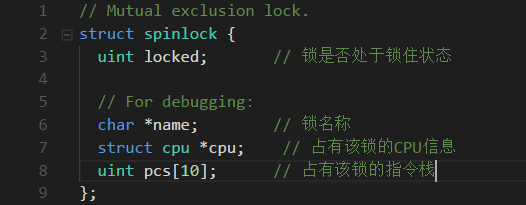
\includegraphics[width=6in]{figures/process/fig6.png}

进程在虚拟内存中的布局如下:

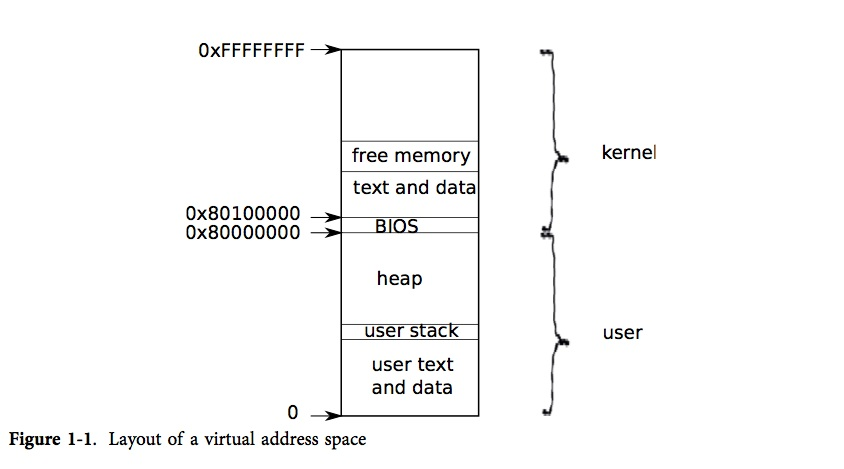
\includegraphics[width=6in]{figures/process/fig7.png}

Xv6使用了一些全局变量来记录进程的状态.
进程数组 proc[NPROC]数组就是进程池。
进程池访问锁 proc\_table\_lock是一个spinlock是用来保护对进程池的临界区访问。
当前运行进程 curproc则是记录每个cpu当前运行的进程。
第一个进程 initproc是记录第一个创立的进程。这个进程十分特殊,它将托管所有没有父进程的进程(也就是父进程先于子进程结束)。
下一进程号 nextid是用来产生进程号的,在系统启动后会一直保持递增。

\subsection{进程的状态}

进程从诞生到死亡要经历若干个阶段,也会有生老病死。简单地说,进程有三种状态:就绪、执行、等待。多种原因可以导致创建一个进程,比如,当操作系统把一个程序从硬盘调入内存后,在开始执行前,操作系统就要为此程序创建一个对应的进程。又比如,一个进程可以自己创建一个子进程,子进程被创建后就是在内存中,处于就绪态,所谓就绪态就是万事具备,只欠CPU这个东风了;一旦进程占有了CPU,就可以执行实际的工作了,其状态就变成了执行态;进程在执行中如果需要等待某个资源(如等硬盘输入数据),则进程会放弃CPU,且其状态就变为等待态,这时操作系统又会从处于就绪态的另一个进程中挑选一个进程占有CPU,则这另一个进程的状态就变成了执行态。当前一个进程所等到数据到来后,处于等待态的前一个进程又被唤醒,并把状态变成为就绪态。

在实际的操作系统中,进程的状态往往多于三种,比如找xv6中,进程具有多种状态,包括:EMBRO, SLEEPING, RUNNABLE, RUNNING和ZOMBIE。定义在proc.h文件中:

\mint{C}{enum proc_state { UNUSED, EMBRYO, SLEEPING, RUNNABLE, RUNNING, ZOMBIE };}

状态的含义如下:

\begin{itemize}
\item UNUSED:进程未被创建(即进程控制块空闲)时的状态;
\item EMBRYO:需要分配一个进程控制块且找到一个处于UNUSED状态的进程控制块时,把此进程控制块状态设置为要使用的状态;
\item SLEEPING:进程由于等待某资源等原因无法执行,进入睡眠状态,即等待态;
\item RUNNABLE:进程获得了除CPU之外的所有资源,处于可运行状态,即就绪态;
\item RUNNING:进程获得CPU,正在运行的状态,即执行态;
\item ZOMBIE:进程结束的状态
\end{itemize}

\subsection{Xv6对于进程的处理过程}

与进程相关的处理函数集中在proc.c中,下面将依次介绍相关处理过程。

\subsubsection{进程管理初始化}

pinit过程仅仅是初始化proc\_table\_lock锁。

\subsubsection{初始化用户进程init}

userinit是初始化第一个用户进程init。其处理过程如下所示:

userinit首先调用allocproc。allocproc(第126行)的工作是在页表中分配一个槽(即结构体 struct proc),并初始化进程的状态,为其内核线程的运行做准备。

allocproc会在proc的表中找到一个标记为 UNUSED的槽位。当它找到这样一个未被使用的槽位后,allocproc 将其状态设置为 EMBRYO,使其被标记为被使用的并给这个进程一个独有的 pid。接下来,它尝试为进程的内核线程分配内核栈。如果分配失败了,allocproc 会把这个槽位的状态恢复为 UNUSED 并返回0以标记失败。

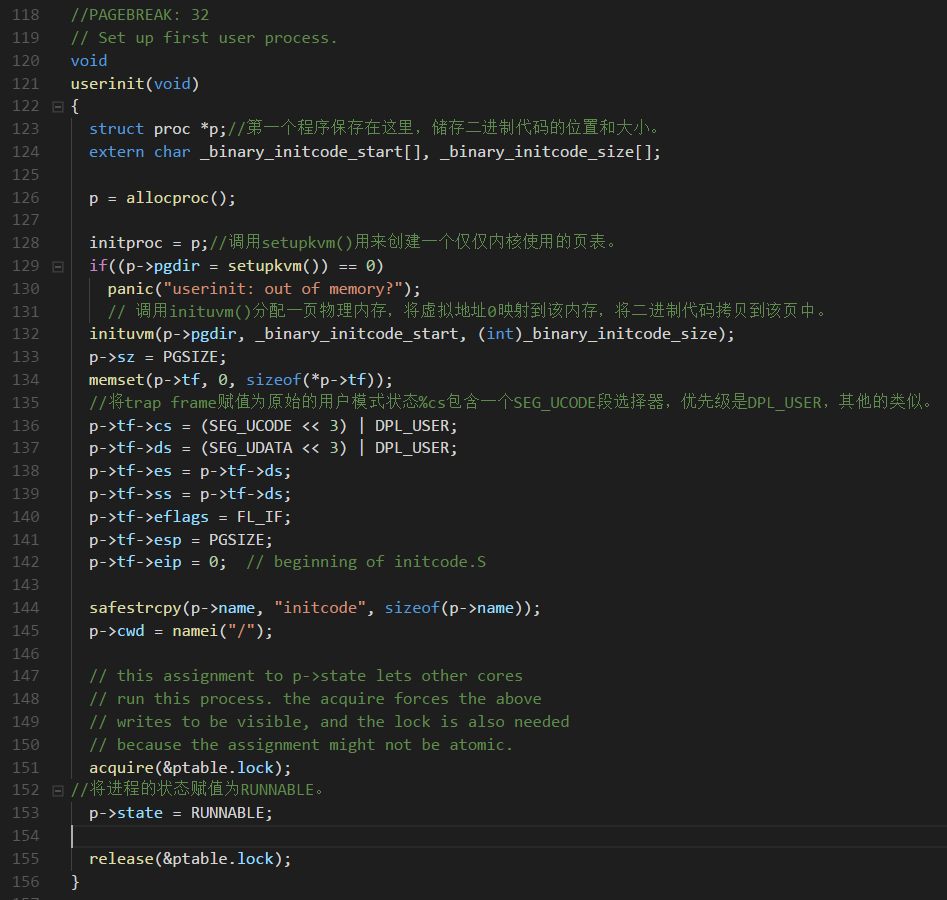
\includegraphics[width=6in]{figures/process/fig8.png}

\subsubsection{创建子进程}

在xv6中,可以通fork来复制父进程内容并创建一个新的子进程。其处理过程如下所示:

一个进程调用 fork() 函数后,系统先给新的进程分配资源,例如存储数据和代码的空间。然后把原来的进程的所有值都复制到新的新进程中,只有少数值与原来的进程的值不同。相当于克隆了一个自己。fork() 函数通过系统调用创建一个与原来进程几乎完全相同的进程,也就是两个进程可以做完全相同的事(即复制了 fork() 函数后的代码),但如果初始参数或者传入的变量不同,两个进程也可以做不同的事。需要注意的是,两个进程拥有不同的内存空间和寄存器(fork()函数之前的变量值是一样的,但存储在不同地方),改变一个进程中的变量不会影响另一个进程。

fork()调用的一个奇妙之处就是它仅仅被调用一次,却能够返回两次,它可能有三种不同的返回值:

\begin{itemize}
\item 在父进程中,fork() 返回新创建子进程的进程pid;
\item 在子进程中,fork() 返回0;
\item 如果出现错误,fork() 返回一个负值;
\end{itemize}

不同的进程有一个唯一的不同进程pid,通过 getpid() 函数可以知道当前进程pid,可以说我们就是通过这个pid知道当前所在进程。

创建新进程成功后,系统中出现两个基本完全相同的进程,这两个进程执行没有固定的先后顺序,哪个进程先执行要看系统的进程调度策略。

\subsubsection{调度进程}

任何操作系统都可能碰到进程数多于处理器数的情况,这样就需要考虑如何分享处理器资源。理想的做法是让分享机制对进程透明。通常我们对进程造成一个自己独占处理器的假象,然后让操作系统的 多路复用机制(multiplex) 将单独的一个物理处理器模拟为多个虚拟处理器。

记下来介绍 xv6 是如何调度进程.
Xv6系统允许有多个cpu,并且每一个cpu获取进程调度的权利是相同的。CPU在scheduler里面进行轮询操作,每次从线程池中选择一个RUNNABLE的进程进行运行。直到运行完毕,或一单位时间片结束,或者进程主动yield或sleep。
进程调度的时机:处于运行状态下的进程如果发生等待事件或者时间耗尽就会被xv6强制终止,变成就绪状态.这样的话,cpu就可以执行其他的进程,提高了cpu的使用率.

Xv6要完成进程切换的功能需要实现从运行中的一个进程切换到另一个进程并且让上下文切换透明化,还有就是xv6支持多个cpu,所以可能出现多个 CPU 同时切换进程的情况,那么我们必须使用一个带锁的方案来避免竞争,最后还有进程退出时必须释放其占用内存与资源.

进程切换:当CPU启动之后,执行scheduler函数,无限循环。在每个周期里,从进程表中找到一个RUNNABLE的进程,切换为进程的上下文,此时开始执行函数。当函数运行结束时,调用return函数,此时切换为CPU的上下文,开始下一循环。

进程唤醒与睡眠:如果一个程序需要等待IO,则CPU会将其设置为睡眠状态,此时不能被执行。当IO信号到达时,执行的进程会将IO信号对应的进程设置为RUNNABLE,即唤醒。下一个scheduler周期的时候,该进程就可能会被执行,处理IO信号。

进程表锁:对于多处理器架构而言,需要用到进程表的时候都需要事先获得表的锁,当结束之后再释放,这样保证了对进程表操作的原子化,可以避免多处理器的竞争问题。

下面通过代码来具体介绍xv6如何实现进程调度部分.
scheduler对每个CPU进行进程调度。CPU到没有运行用户进程时,就会进入这个过程中。这个过程不停的从进程中选出一个RUNNABLE的进程,然后运行这个进程(通过swtch.S中的swtch函数进行)。

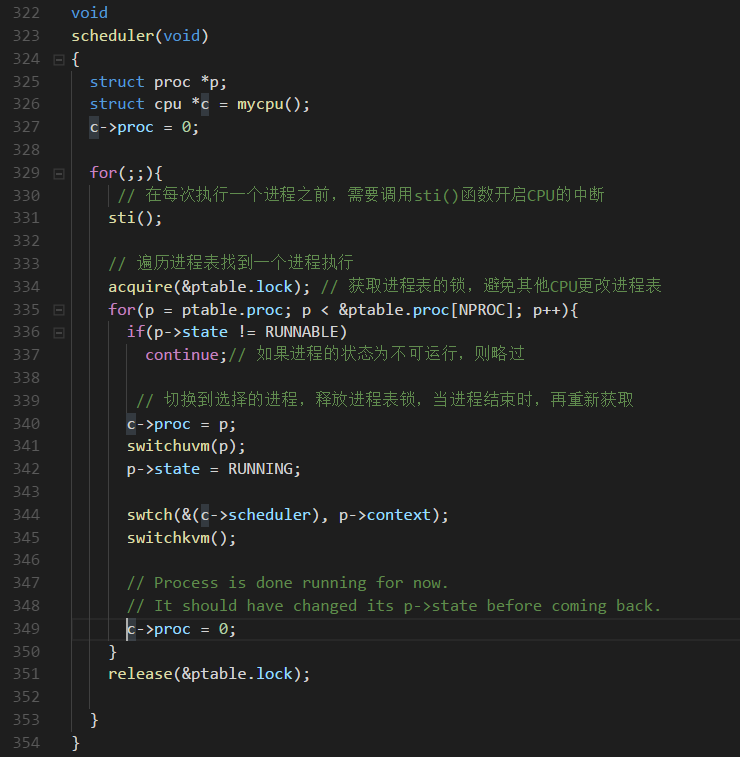
\includegraphics[width=6in]{figures/process/fig9.png}

sched是放弃当前的用户进程,进入scheduler()。只需用通过swtch进行上下文切换即可。

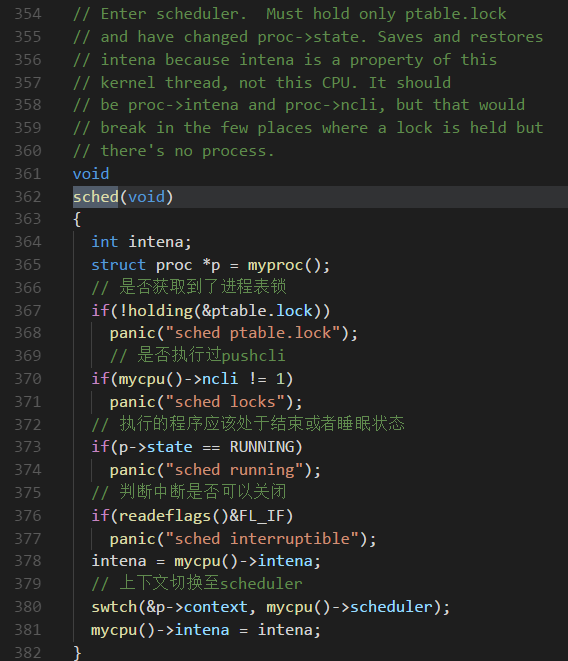
\includegraphics[width=6in]{figures/process/fig10.png}

\subsubsection{设置用户进程返回}

forkret是用于新fork的进程进行返回地址用的。由于调用sys\_fork创建的新进程是通过shceduler()调用的,因此运行之前需要把proc\_table\_lock锁释放。

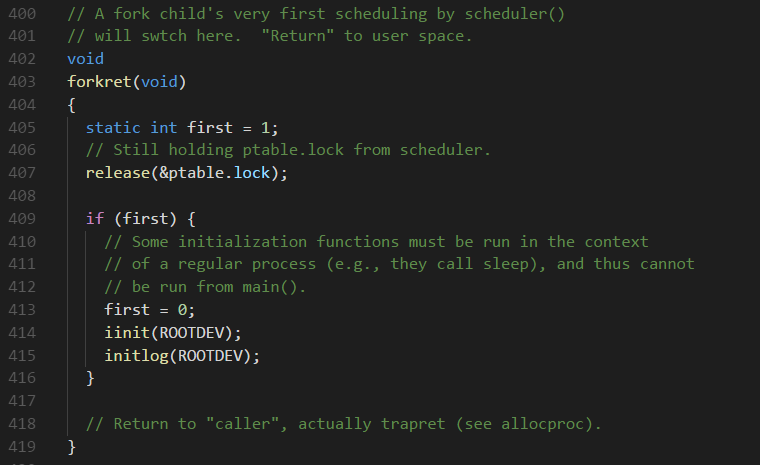
\includegraphics[width=6in]{figures/process/fig11.png}

sleep功能是让进程休眠。首先获得proc\_table\_lock,然后将记录chan,也就是说只有相关的chan才能把其唤起。然后调用sched()。当期被唤醒是,将继续运行,此时将chan等记录清空,并且将proc\_table\_lock锁释放,而获得lk锁。

\subsubsection{睡眠进程}

sleep功能是让进程休眠。首先获得proc\_table\_lock,然后将记录chan,也就是说只有相关的chan才能把其唤起。然后调用sched()。当期被唤醒是,将继续运行,此时将chan等记录清空,并且将proc\_table\_lock锁释放,而获得lk锁。

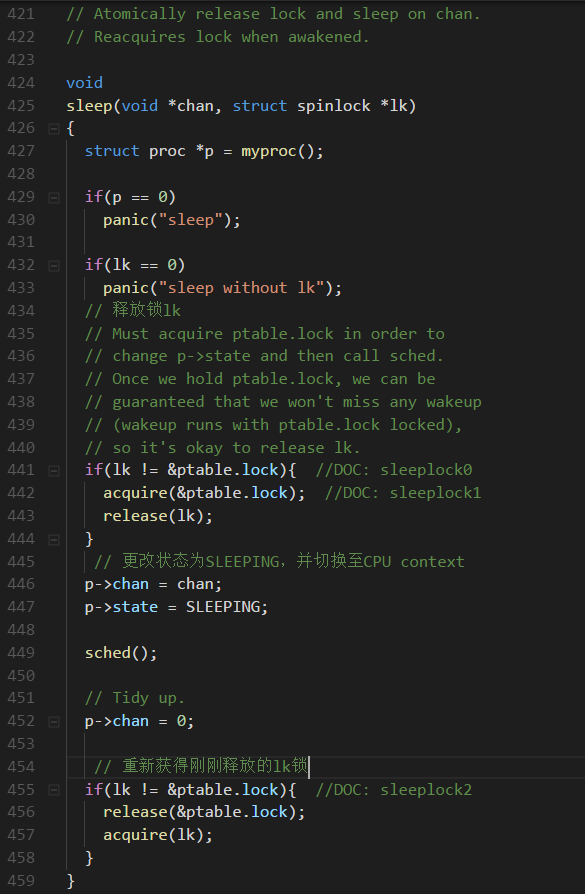
\includegraphics[width=6in]{figures/process/fig12.png}

\subsubsection{唤醒进程}

值得注意的是,使进程进入睡眠需要两个锁,lk和ptable.lock,由于之前已经得到了ptable.lock,所以wakeup在此期间不会执行,直至进程完全进入睡眠状态,所以lk这个锁可以释放。
wakeup函数的主体部分位于wakeup1函数中。

wakeup功能是唤醒进程。先获取proc\_table\_lock,然后调用函数wakeup1,然后释放proc\_table\_lock。

wakeup1是将由于chan休眠的进程都唤醒,即把进程的状态由SLEEPING改成RUNNABLE。

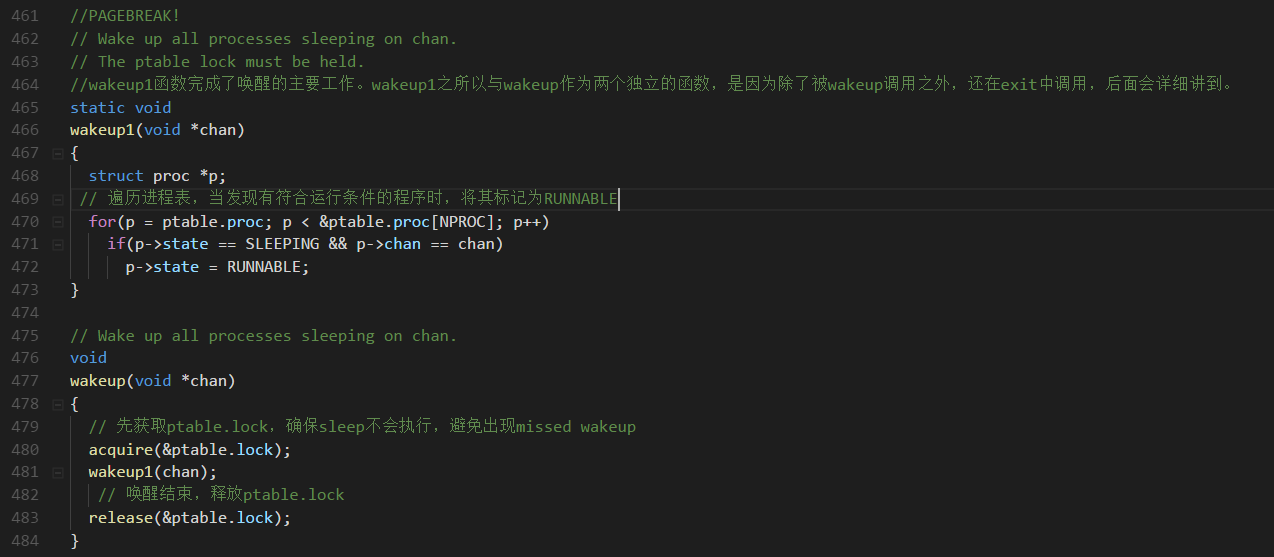
\includegraphics[width=6in]{figures/process/fig13.png}

\subsubsection{杀死进程}

kill的作用是杀死某个进程。只需要从进程池中找到拥有相应进程ID的进程,将其killed状态置1即可。如果目标进程出于sleeping状态则将其设置成RUNNABLE使其尽早被杀掉。

详细的代码如下所示.

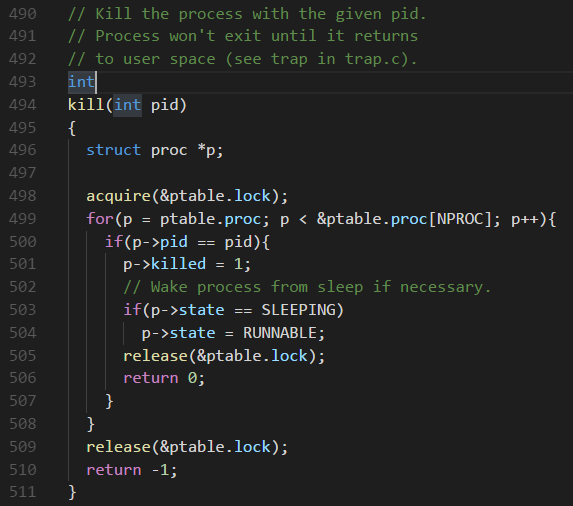
\includegraphics[width=6in]{figures/process/fig14.png}

\subsubsection{退出进程}

exit完成了进程结束时的资源释放以及子进程处理等工作。在退出之前,用户进程需要关闭打开的文件(238-243行),将打开的文件夹关闭(358~359)。同时唤醒父进程,因为其可能出于wait状态。并将其子进程托管于init。然后改变其状态为ZOMBIE(等待父进程进行回收)。最后调用sched放弃CPU。

  \subsubsection{等待进程结束}

  wait是用于父进程等待子进程结束只用的。做法是不断的循环知道找到一个子进程变成ZOMBIE状态,则释放ZOMBIE子进程(回收其资源),然后结束循环返回其子进程的进程ID。在循环的时候需要判断是否被外部进程Kill,或有无活跃子进程,如果被杀死或无活跃子进程,则推出循环。

  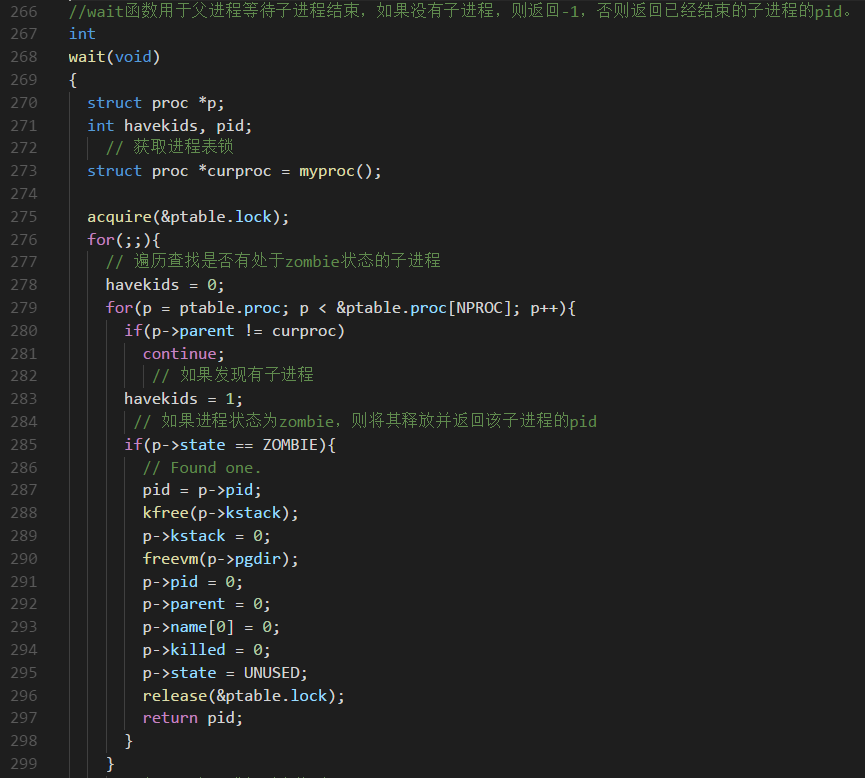
\includegraphics[width=6in]{figures/process/fig16.png}
